\documentclass[tikz,margin=5mm]{standalone}
\usepackage{amssymb}
\usetikzlibrary{shapes.multipart,positioning,arrows,calc}
\tikzset{
    listnode/.style={
        rectangle split,rectangle split parts=2,draw,rectangle split horizontal,fill=yellow!15
    },
    startnode/.style={
        draw,minimum width=1cm,minimum height=.75cm
    }
}
\begin{document}
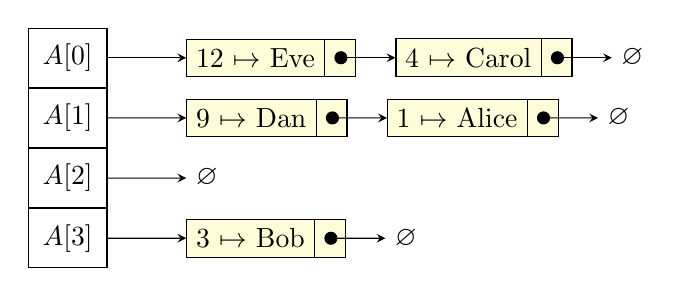
\begin{tikzpicture}[scale=.2, >=stealth]
\node[startnode] (t0) {$A[0]$};
\node[startnode,below=0pt of t0] (t1) {$A[1]$};
\node[startnode,below=0pt of t1] (t2) {$A[2]$};
\node[startnode,below=0pt of t2] (t3) {$A[3]$};
\node[listnode,right=of t0] (eve) {12 $\mapsto$ Eve};
\node[listnode,right=.5cm of eve] (carol) {4 $\mapsto$ Carol};
\node[listnode,right=of t1] (dan) {9 $\mapsto$ Dan};
\node[listnode,right=.5cm of dan] (alice) {1 $\mapsto$ Alice};
% \node[listnode,right=of t2] (2a) {2};
% \node[listnode,right=.5cm of 2a] (5a) {5};
% \node[listnode,right=.5cm of 5a] (8a) {8};
\node[listnode,right=of t3] (bob) {3 $\mapsto$ Bob};
\node[right=.5cm of carol] (carolx) {$\varnothing$};
\node[right=.5cm of alice] (alicex) {$\varnothing$};
\node[right=of t2] (t2x) {$\varnothing$};
\node[right=.5cm of bob] (bobx) {$\varnothing$};
% \node[right=.5cm of 8a] (8x) {$\varnothing$};
\draw[*->] let \p1 = (eve.two), \p2 = (eve.center) in (\x1,\y2) -- (carol);
\draw[*->] let \p1 = (carol.two), \p2 = (carol.center) in (\x1,\y2) -- (carolx);
\draw[*->] let \p1 = (dan.two), \p2 = (dan.center) in (\x1,\y2) -- (alice);
\draw[*->] let \p1 = (alice.two), \p2 = (alice.center) in (\x1,\y2) -- (alicex);
\draw[*->] let \p1 = (bob.two), \p2 = (bob.center) in (\x1,\y2) -- (bobx);
% \draw[*->] let \p1 = (2a.two), \p2 = (2a.center) in (\x1,\y2) -- (5a);
% \draw[*->] let \p1 = (5a.two), \p2 = (5a.center) in (\x1,\y2) -- (8a);
% \draw[*->] let \p1 = (8a.two), \p2 = (8a.center) in (\x1,\y2) -- (8x);
\draw[->] (t0) edge (eve) (t1) edge (dan) (t2) edge (t2x) (t3) edge (bob);
\end{tikzpicture}
\end{document}
    
